% !TEX encoding = UTF-8 Unicode

\textbf{Defina formalmente, através de expressões regulares sobre o conjunto de caracteres ASCII, a sintaxe de cada um dos tipos de átomos a serem extraídos do texto-fonte pelo analisador léxico, bem como de cada um dos espaçadores e comentários.}

\begin{itemize}

	\item DELIM: \verb!/[{}()\[\];]/!
	
	\begin{figure}[H]
		\centering 
		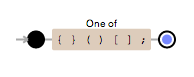
\includegraphics{images/REGEX/1-DELIM.png}  
		\caption{Expressão Regular DELIM}
	\end{figure}
	
	\item SPACE: \verb!/[ \t\r\n\v\f]+/!
	
	\begin{figure}[H]
		\centering 
		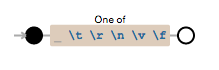
\includegraphics{images/REGEX/2-SPACE.png}  
		\caption{Expressão Regular SPACE}
	\end{figure}
	
	\item COMMENT: \verb!/#[^\n]*/!
	
	\begin{figure}[H]
		\centering 
		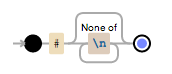
\includegraphics{images/REGEX/3-COMMENT.png}  
		\caption{Expressão Regular COMMENT}
	\end{figure}
	
	\item IDENT: \verb!/[a-zA-Z_][a-zA-Z0-9_]*/!
	
	\begin{figure}[H]
		\centering 
		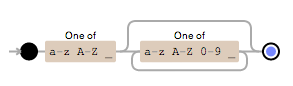
\includegraphics{images/REGEX/4-IDENT.png}  
		\caption{Expressão Regular IDENT}
	\end{figure}
	
	\item INTEGER: \verb!/[0-9]+/!
	
	\begin{figure}[H]
		\centering 
		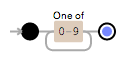
\includegraphics{images/REGEX/5-INTEGER.png}  
		\caption{Expressão Regular INTEGER}
	\end{figure}
	
	\item FLOAT: \verb!/[0-9]*\.[0-9]+/!
	
	\begin{figure}[H]
		\centering 
		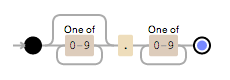
\includegraphics{images/REGEX/6-FLOAT.png}  
		\caption{Expressão Regular FLOAT}
	\end{figure}
	
	\item CHAR: \verb!/'(?:\\[abtnvfre\\]|[\x20-\x5B\x5D-\x7E])?'/!
	
	\begin{figure}[H]
		\centering 
		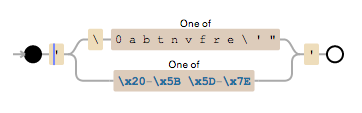
\includegraphics{images/REGEX/7-CHAR.png}  
		\caption{Expressão Regular CHAR}
	\end{figure}
	
	\item STRING: \verb!/"(?:\\"|[^"])*"/!
	
	\begin{figure}[H]
		\centering 
		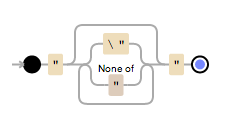
\includegraphics{images/REGEX/8-STRING.png}  
		\caption{Expressão Regular STRING}
	\end{figure}
	
	\item OPER: \verb!/[\+\-\*\/%=!<>][=]?/!
	
	\begin{figure}[H]
		\centering 
		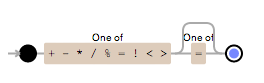
\includegraphics{images/REGEX/9-OPER.png}  
		\caption{Expressão Regular OPER}
	\end{figure}

\end{itemize}
